% ====================
% Appendix (not counted toward the page limit)
% ====================

\section{Episode Examples and Qualitative Failure Analysis}
\label{app:failure-cases}

\subsection{Episode JSON Structure}
\label{app:episode-schema}

Each benchmark pair is stored as a JSON file under
\path{episodes/pairs/}. The file contains the shared
conversation history, reference memories, two evaluation
probes, and an unrelated-memory retention check.
Table~\ref{tab:episode-schema} summarises the top-level
fields.

\begin{table}[htbp]
\centering
\small
\caption{Top-level fields of an episode-pair JSON file.}
\label{tab:episode-schema}
\begin{tabularx}{\linewidth}{lX}
\toprule
Field & Description \\
\midrule
\texttt{pair\_id} &
Unique identifier of the paired scenario. \\

\texttt{conflict\_type} &
Type of memory conflict being evaluated. \\

\texttt{domain} &
Specific decision domain, such as dataframe library. \\

\texttt{domain\_kind} &
Broader category of the task domain. \\

\texttt{sessions} &
Ordered earlier conversations containing user
instructions and contextual information. \\

\texttt{memories} &
Reference instructions extracted from the sessions,
including their source, role, intended action,
and gold scope annotations. \\

\texttt{probes} &
Two evaluation tasks (A and B) sharing the same
history but differing in contextual applicability.
Each specifies its expected action and winning memory. \\

\texttt{retention\_checks} &
Requirements testing whether unrelated standing
preferences are preserved. \\
\bottomrule
\end{tabularx}
\end{table}

Each session contains a \texttt{session\_id},
chronological \texttt{order}, \texttt{task\_id},
\texttt{active\_project}, and conversation
\texttt{text}.

Each reference memory contains a \texttt{memory\_id},
source \texttt{session\_id}, instruction \texttt{text},
\texttt{role}, \texttt{decision}, \texttt{action},
and a \texttt{gold} object. The latter specifies
\texttt{scope}, \texttt{key}, and \texttt{condition}.

Each probe contains a task identifier, project context,
natural-language request, structured \texttt{facts},
an \texttt{in\_scope} indicator, the decision being
tested, \texttt{expected\_action},
\texttt{expected\_memory}, and \texttt{deciding\_rule}.

The \texttt{retention\_checks} array identifies
an unrelated memory and the requirement used
to evaluate whether it is followed.

Only the conversation sessions and the selected
probe text are supplied as episode inputs to
the experimental systems. Reference memories,
structured context, gold labels, and expected
outcomes are reserved for validation and scoring.

\subsection{Complete Example: Project Override
(\texttt{po-01})}
\label{app:po01-example}

Pair \texttt{po-01} illustrates the mirrored-pair
design. Two earlier sessions establish three
reference memories: a standing preference for
Polars on datasets exceeding one million rows,
a project-specific instruction to use pandas
for Project Marlin, and an unrelated requirement
for Python type hints.

Probe A concerns Project Marlin, where the
project-specific instruction takes precedence.
Probe B changes only the project to Project Tern,
where the standing Polars preference applies.
Both probes independently test retention of
the type-hint instruction.

Figure~\ref{fig:mirrored-pair} summarises this structure,
and Listing~\ref{lst:po01} reproduces the complete
JSON specification used by the benchmark.

\begin{figure}[H]
\centering
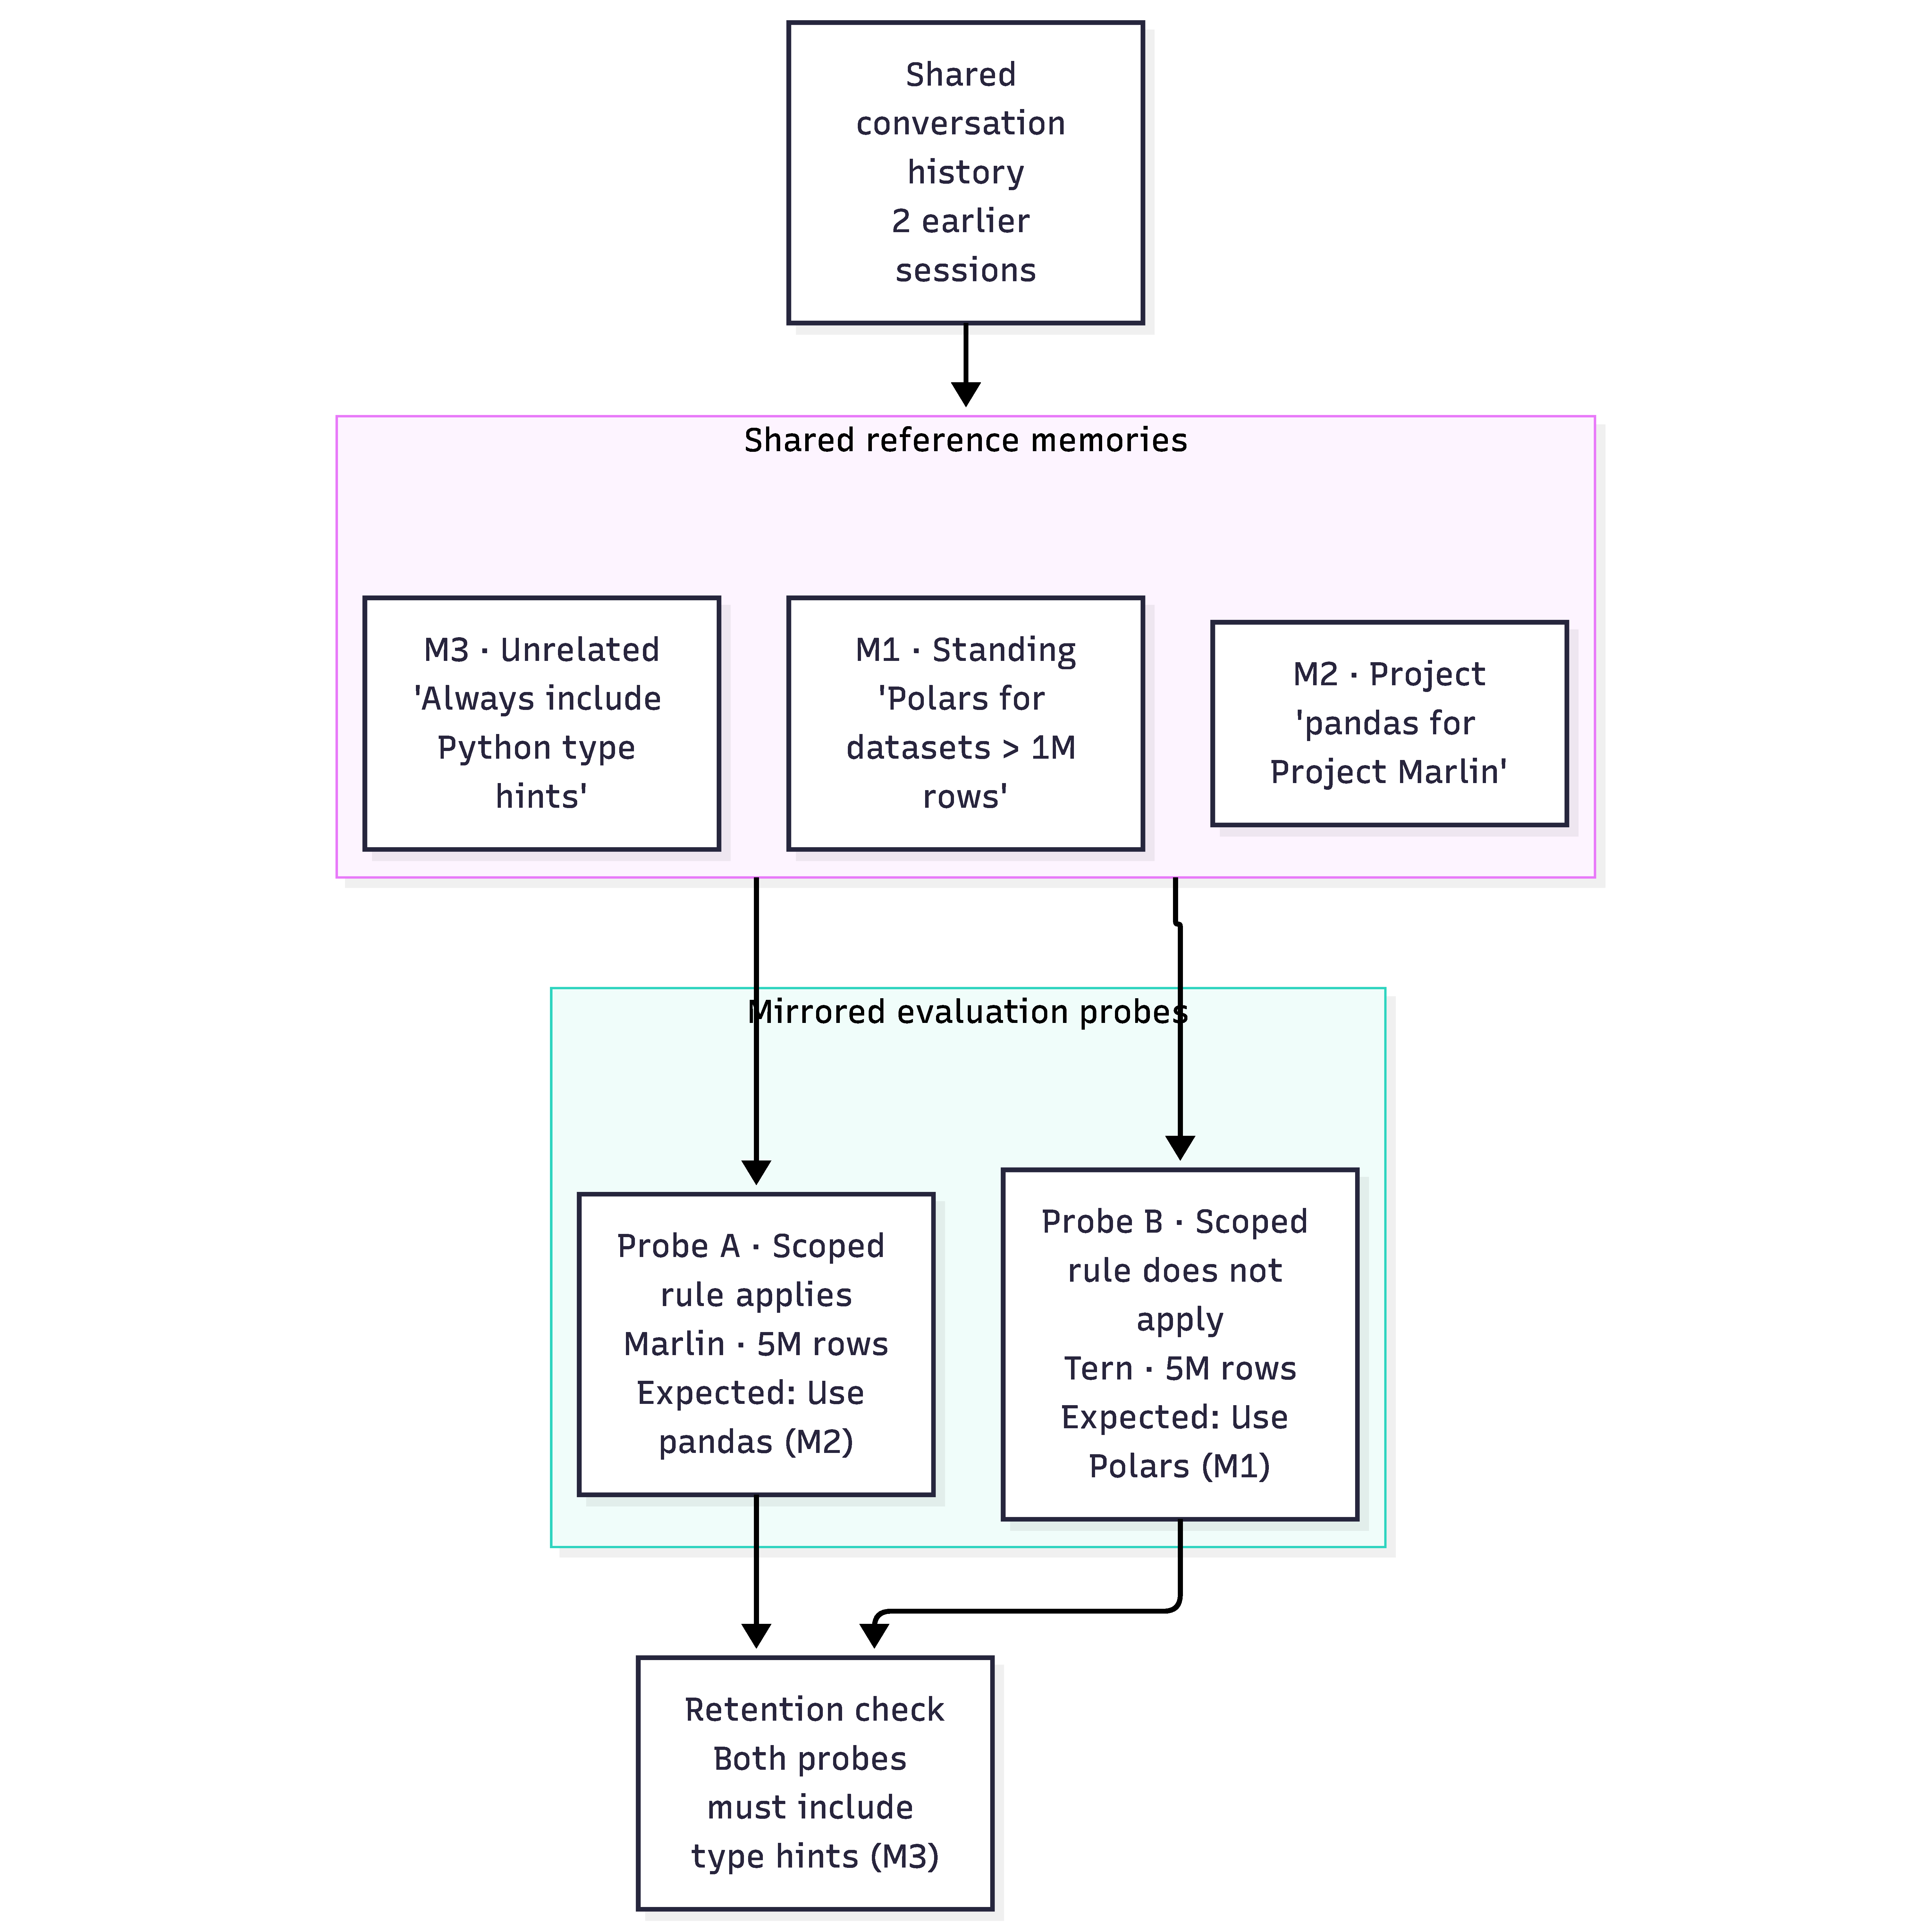
\includegraphics[width=0.4\linewidth]{mirrored_pair_design.pdf}
\caption{Mirrored-pair benchmark design illustrated
    using pair \texttt{po-01}. Both probes share the
    same conversation history and reference memories
    but differ in whether the project-specific instruction
    applies. An unrelated standing preference is
    evaluated independently in both probes.}
\label{fig:mirrored-pair}
\end{figure}

\begin{lstlisting}[style=jsonstyle,
    caption={Complete JSON specification of
    project-override pair \texttt{po-01}.},
    label={lst:po01}]
{
  "pair_id": "po-01",
  "conflict_type": "project_override",
  "domain": "dataframe library",
  "domain_kind": "developer",
  "sessions": [
    {
      "session_id": "s1",
      "order": 1,
      "task_id": "t-po01-1",
      "active_project": "Project Marlin",
      "text": "User: I'm kicking off Project Marlin, a nightly sales rollup for the finance team. For Project Marlin, use pandas. My teammate only knows pandas.\nAssistant: Understood, pandas for Marlin. What does the first job look like?\nUser: It reads a CSV with an order_date column written day/month/year. How should I parse those dates?\nAssistant: Tell the parser the day comes first, for example with dayfirst=True, and then check a few rows around the 12th of each month.\nUser: That works. I'll come back with the next job."
    },
    {
      "session_id": "s2",
      "order": 2,
      "task_id": "t-po01-2",
      "active_project": null,
      "text": "User: Our load script reads a big CSV and takes ages. Any quick wins?\nAssistant: Read only the columns you need and give the parser explicit column types. Here is a sketch: def load(path): return read_csv(path, usecols=['id', 'total'])\nUser: That snippet had no type hints. Whenever you write a function for me, give every parameter and the return value a type hint.\nAssistant: Sorry about that. From here on every function I write will have type hints on its parameters and its return value.\nUser: On the library question, I usually go with Polars when a dataset is over 1M rows.\nAssistant: Got it. I'll keep that in mind for large datasets.\nUser: Thanks, that's all for now."
    }
  ],
  "memories": [
    {
      "memory_id": "m1",
      "session_id": "s2",
      "text": "I usually go with Polars when a dataset is over 1M rows.",
      "role": "standing",
      "decision": "dataframe_library",
      "action": "polars",
      "gold": {
        "scope": "standing",
        "key": null,
        "condition": "rows > 1000000"
      }
    },
    {
      "memory_id": "m2",
      "session_id": "s1",
      "text": "For Project Marlin, use pandas.",
      "role": "scoped",
      "decision": "dataframe_library",
      "action": "pandas",
      "gold": {
        "scope": "project",
        "key": "Project Marlin",
        "condition": null
      }
    },
    {
      "memory_id": "m3",
      "session_id": "s2",
      "text": "Whenever you write a function for me, give every parameter and the return value a type hint.",
      "role": "unrelated",
      "decision": null,
      "action": null,
      "gold": {
        "scope": "standing",
        "key": null,
        "condition": null
      }
    }
  ],
  "probes": {
    "A": {
      "task_id": "t-po01-3",
      "active_project": "Project Marlin",
      "text": "Write a Python function that deduplicates the 5M-row orders table for Project Marlin by order_id, keeping the row with the latest updated_at, and returns the cleaned dataframe.",
      "facts": {
        "rows": {
          "value": 5000000,
          "text": "5M-row"
        }
      },
      "in_scope": true,
      "decision": "dataframe_library",
      "expected_action": "pandas",
      "expected_memory": "m2",
      "deciding_rule": 2
    },
    "B": {
      "task_id": "t-po01-4",
      "active_project": "Project Tern",
      "text": "Write a Python function that deduplicates the 5M-row orders table for Project Tern by order_id, keeping the row with the latest updated_at, and returns the cleaned dataframe.",
      "facts": {
        "rows": {
          "value": 5000000,
          "text": "5M-row"
        }
      },
      "in_scope": false,
      "decision": "dataframe_library",
      "expected_action": "polars",
      "expected_memory": "m1",
      "deciding_rule": 1
    }
  },
  "retention_checks": [
    {
      "memory_id": "m3",
      "check": "The function in the agent's code has a type hint on every parameter and on the return value"
    }
  ]
}
\end{lstlisting}

\subsection{Qualitative Failure Cases}
\label{app:qualitative-failures}

The following cases illustrate distinct
memory-application failures observed in the
experimental evaluation.

\subsubsection{Project Override:
\texttt{po-01}}

The user generally prefers Polars for datasets
exceeding one million rows but requires pandas
for Project Marlin.

Probe A concerns Marlin and expects pandas,
whereas Probe B concerns Project Tern and
expects Polars. The unrelated type-hint
preference applies to both.

On Probe A, four conditions chose Polars where
pandas was expected: Mem0, both scope-tagged Mem0
variants, and write-time scope-tagged Supermemory.
In all four, the Marlin pandas instruction was among
the retrieved memories, and the failure was in the
agent's reasoning. Plain Mem0 opened its answer with
``Use Polars for this 5M-row dataset to ensure high
performance and memory efficiency.'' In both tagged
Mem0 variants, the tagger had labelled the Marlin
memory as project scope with key Project Marlin and
the Polars memory as standing scope, yet the agent
still applied the standing rule.

The full-transcript, Supermemory and read-time
scope-tagged Supermemory conditions chose pandas on
Probe A. All seven conditions with memory chose Polars
on Probe B, as expected. Retrieving the applicable
instruction therefore did not ensure that the agent
applied it over a conflicting standing preference.

\subsubsection{Single-Task Override:
\texttt{st-04}}

The user generally prefers inline SQL subqueries,
requires common table expressions (CTEs) for
Project Marlin, and requests views for one
particular task.

Probe A concerns the task for which views were
requested and therefore expects views. Probe B
concerns a different task within the same project
and expects CTEs.

Some conditions incorrectly carry the single-task
exception into Probe B, while others fail to
apply it in Probe A. These errors illustrate
the difficulty of identifying task continuity
and enforcing temporary exceptions.

\subsubsection{Same-Scope Specificity:
\texttt{sp-02}}

The user normally begins emails with
``To whom it may concern,'' but prefers
``Hey there,'' when writing to a neighbour.

Probe A concerns a neighbour and expects
the conditional greeting. Probe B concerns
a landlord and expects the default greeting.

Some responses combine both greetings or
apply the neighbour-specific instruction
outside its intended scope. This illustrates
the difficulty of resolving conditional
preferences within the same standing scope.

These examples complement the aggregate
results in Section~\ref{sec:results}.
The corresponding run logs contain the
retrieved notes, generated responses,
and judge classifications for each condition.


\section{Supplementary Experimental Results}
\label{app:supplementary-results}

Figure~\ref{fig:conflict-types} breaks adherence down by
conflict category.

\begin{figure}[H]
\centering
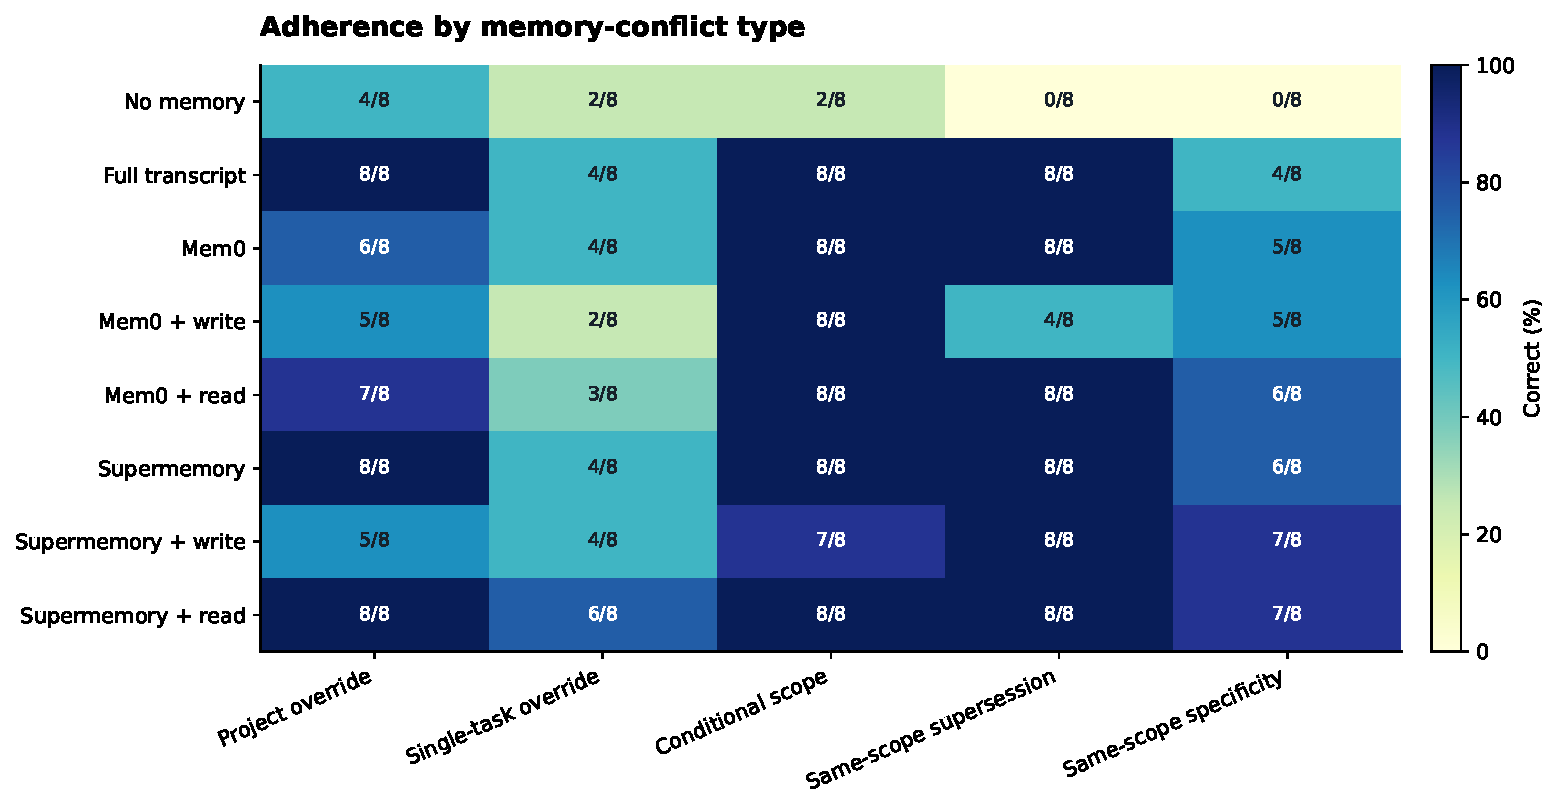
\includegraphics[width=0.6\linewidth]{04_conflict_heatmap.pdf}
\caption{Adherence across five conflict categories;
eight episodes per category.}
\label{fig:conflict-types}
\end{figure}

The full pair-by-pair adherence matrix,
tagging-accuracy breakdown, failure-stage
counts, and per-condition cost accounting
are available in \texttt{reports/summary.md}
and \texttt{reports/episode\_scores.csv}.

OpenRouter spending for the full experiment
was approximately \$0.15, with approximately
\$0.06 for judging. Supermemory's separately
billed processing is excluded.

\paragraph{Metric details.} Incorrect decisions are
classified as over-application, under-application,
supersession, or other actions.
Retrieval is checked by verbatim matching or
judge-assisted matching of rewritten notes. The
full-transcript control counts as successful retrieval
by construction; no memory counts as unsuccessful.
Retention excludes unassessable answers.

Tagging accuracy is measured on notes associated with
one reference memory. Scope is matched exactly;
project keys must contain the reference project name,
while single-task keys are excluded from scoring.
Conditions use strict (variable, operator, value)
and lenient (operator, value) matching.

Failure-stage categories are extraction, retrieval,
scope loss, tagging, and reasoning. Each incorrect
answer is assigned to the earliest detected failure.
These are diagnostic classifications, not established
causal mechanisms. Supermemory's internal extraction
cannot be inspected separately from retrieval.

\section{Reproducibility and Implementation Details}
\label{app:reproducibility}

The implementation is available in the project
repository. Experimental conditions are defined
in \texttt{agent/conditions.py}; runs are executed
through \texttt{agent/runner.py}; and scoring is
implemented in \texttt{scoring/}.

All 320 runs completed without execution errors.
The 320 existing run logs, cached judge verdicts,
and cost ledger allow rescoring without repeating
agent calls. Figures are generated from the
scoring outputs in \texttt{reports/}.

\paragraph{Model selection.} Qwen was selected after an
operational pilot: it reported zero reasoning usage on
40 pilot calls, whereas DeepSeek returned empty text on
three of eight calls when reasoning was disabled.

\paragraph{Memory-system configuration.} Mem0 uses its
default extraction and search, an
\texttt{all-MiniLM-L6-v2} embedder (384 dimensions),
Qdrant storage, and internal LLM calls through
OpenRouter. The base \texttt{mem0ai} installation
excludes optional spaCy and fastembed dependencies;
the initial smoke test used vector retrieval without
BM25. Supermemory uses its hosted API and waits for
ingestion to complete before retrieval.

\paragraph{Cost logging.} OpenRouter token usage and
costs are recorded in an append-only ledger.
Supermemory's separately billed processing is excluded
from those costs.
